\section{Requirements Captured}
The following are requirement divided into functional and non-functional requirement which where collected after consulting with the client.
\subsection*{Functionality requirements}
The list of the requirements for the application where as follows:
\newline\textbf{Functional Requirements}
\begin{itemize}
	\item Rendering of the map on the user screen
	\item Have signal strength indicators on the map. These should be updated on a real-time basis.
	\item Save signal strength on the database for a specific location.
	\item Zoom in and zoom out of the campus map
\end{itemize}
\textbf{Non-Functional Requirements}
\begin{itemize}
	\item Real-time receiving of data being updated in the database.
	\item Speed up on the rendering of the areas and their strengths on the map.
\end{itemize}



The next section deals with the analysis of your system. Cover the
functional, non-functional and usability requirements. This is where
you present your use case narratives and diagrams. 

Discuss the major analysis artefacts that you produced. We will expect
you to produce at least one overall description of the architecture
used in your system as a diagram, either here or below (see Section
\ref{ss:design-overview}). You may also want to include an analysis
class hierarchy diagram.

\subsection{Design Overview}
\label{ss:design-overview}

The next section is an overview of your design. The system design has
to be justified in terms of the expected behaviour of the final
product. 

If you produced a design class diagram put it here.

\begin{figure}[h!]
  \center{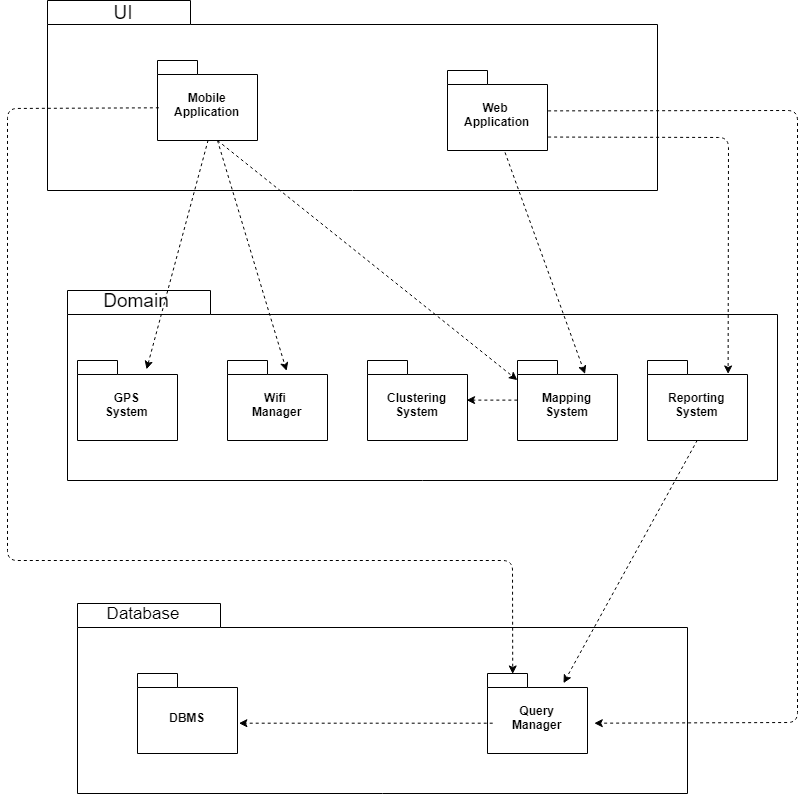
\includegraphics[scale=0.8]{images/architecture.png}}
  \caption{An architecture diagram. Caption to go below figure}
  \label{fig:architecture}
\end{figure}

You must present the overall architecture of the system together with
an architecture diagram. You may choose what kind of diagram best
suits your project but we would expect a layered architecture diagram
(see Figure \ref{fig:architecture}) unless there is a good reason for
some other kind of diagram. It need not be a formal UML diagram as
long as it conveys all the necessary information clearly.

You should then (in subsections) cover the algorithms and the data
organisation used and why they were considered the best. 

